\PassOptionsToPackage{unicode=true}{hyperref} % options for packages loaded elsewhere
\PassOptionsToPackage{hyphens}{url}
%
\documentclass[ignorenonframetext,aspectratio=43,]{beamer}

\setbeamercovered{dynamic}
\usepackage[spanish]{babel}
\selectlanguage{spanish}
\uselanguage{Spanish}
\languagepath{Spanish}

\usepackage{pgfpages}
\setbeamertemplate{caption}[numbered]
\setbeamertemplate{caption label separator}{: }
\setbeamercolor{caption name}{fg=normal text.fg}
\beamertemplatenavigationsymbolsempty
% Prevent slide breaks in the middle of a paragraph:
\widowpenalties 1 10000
\raggedbottom
\setbeamertemplate{part page}{
\centering
\begin{beamercolorbox}[sep=16pt,center]{part title}
  \usebeamerfont{part title}\insertpart\par
\end{beamercolorbox}
}
\setbeamertemplate{section page}{
\centering
\begin{beamercolorbox}[sep=12pt,center]{part title}
  \usebeamerfont{section title}\insertsection\par
\end{beamercolorbox}
}
\setbeamertemplate{subsection page}{
\centering
\begin{beamercolorbox}[sep=8pt,center]{part title}
  \usebeamerfont{subsection title}\insertsubsection\par
\end{beamercolorbox}
}
\AtBeginPart{
  \frame{\partpage}
}
\AtBeginSection{
  \ifbibliography
  \else
    \frame{\sectionpage}
  \fi
}
\AtBeginSubsection{
  \frame{\subsectionpage}
}
\usepackage{lmodern}
\usepackage{amssymb,amsmath}
\usepackage{ifxetex,ifluatex}
\usepackage{fixltx2e} % provides \textsubscript
\ifnum 0\ifxetex 1\fi\ifluatex 1\fi=0 % if pdftex
  \usepackage[T1]{fontenc}
  \usepackage[utf8]{inputenc}
  \usepackage{textcomp} % provides euro and other symbols
\else % if luatex or xelatex
  \usepackage{unicode-math}
  \defaultfontfeatures{Ligatures=TeX,Scale=MatchLowercase}
\fi
\usetheme[]{metropolis}
% use upquote if available, for straight quotes in verbatim environments
\IfFileExists{upquote.sty}{\usepackage{upquote}}{}

\IfFileExists{parskip.sty}{%
\usepackage{parskip}
}{% else
\setlength{\parindent}{0pt}
\setlength{\parskip}{6pt plus 2pt minus 1pt}
}
\usepackage{hyperref}
\hypersetup{
            pdftitle={Modelos de computación cuánticos},
            pdfauthor={Pablo Baeyens Fernández},
            pdfborder={0 0 0},
            breaklinks=true}
\urlstyle{same}  % don't use monospace font for urls
\newif\ifbibliography
\setlength{\emergencystretch}{3em}  % prevent overfull lines
\providecommand{\tightlist}{%
  \setlength{\itemsep}{0pt}\setlength{\parskip}{0pt}}
\setcounter{secnumdepth}{0}

% set default figure placement to htbp
\makeatletter
\def\fps@figure{htbp}
\makeatother

\setsansfont[
    Extension      = .otf,
    UprightFont    = *-Light,
    ItalicFont     = *-LightItalic,
    BoldFont       = *-Regular,
    BoldItalicFont = *-RegularItalic
]{FiraSans}
\setmonofont[
    Extension   = .otf,
    UprightFont = *-Regular,
    BoldFont    = *-Medium
]{FiraMono}

\usepackage{appendixnumberbeamer}
\usepackage{svg}
\metroset{titleformat=smallcaps, sectionpage=progressbar, progressbar=frametitle, block=fill}
\definecolor{AzulUGR}{HTML}{007FC0}
\definecolor{RojoUGR}{HTML}{CB2C30}
\setbeamercolor{alerted text}{fg=AzulUGR}
\setbeamercolor{frametitle}{bg=RojoUGR}

\usepackage{tikz}
\usetikzlibrary{arrows}


\newtheorem{teorema}{Teorema}
\newtheorem{corolario}{Corolario}
\newtheorem{lema}{Lema}
\newtheorem{definicion}{Definición}
\newtheorem{problema}{Problema}
\newtheorem{proposicion}{Proposición}
\newtheorem{principio}{Principio}
\newtheorem{ejemplo}{Ejemplo}
\newtheorem{algoritmo}{Algoritmo}

% Bra-ket notation
\newcommand{\bra}[1]{\left\langle#1\right|}
\newcommand{\ket}[1]{\left|#1\right\rangle}
\newcommand{\bk}[2]{\langle #1|#2\rangle}

% Basic commands
\newcommand{\NN}{\mathbb{N}}
\newcommand{\ZZ}{\mathbb{Z}}
\newcommand{\RR}{\mathbb{R}}
\newcommand{\CC}{\mathbb{C}}
\newcommand{\BB}{\mathbb{B}}
\newcommand{\PC}{\mathbb{P}\mathbb{C}}
\newcommand{\norm}[1]{\left\lVert#1\right\rVert}
\newcommand{\set}[2]{\left\{ #1 \;:\; #2 \right\}}

% Complexity
\newcommand{\talph}{\mathcal{T}}
\newcommand{\blank}{\square}
\newcommand{\ew}{\varepsilon}
\newcommand{\TIME}{\operatorname{TIME}}
\newcommand{\SPACE}{\operatorname{SPACE}}
\newcommand{\NTIME}{\operatorname{NTIME}}
\newcommand{\NSPACE}{\operatorname{NSPACE}}
\newcommand{\SIZE}{\operatorname{SIZE}}
\newcommand{\poly}{\operatorname{poly}}
\newcommand{\qeq}{\overset{?}{=}}


\usepackage{listings}

\definecolor{backg}{HTML}{F2F2F2} % Fondo
\definecolor{comments}{HTML}{a8a8a8} % Comentarios
\definecolor{keywords}{HTML}{08388c} % Palabras clave
\definecolor{strings}{HTML}{0489B1}  % Strings

\lstset{
language=haskell,
basicstyle=\small\ttfamily,
breaklines=true,
keywordstyle=\color{keywords},
commentstyle=\color{comments},
stringstyle=\color{strings},
morekeywords={*,Qubit,Circ,QShape,Oracle,QDInt,pure,...},
tabsize=2,
% Acentos, ñ, ¿, ¡ (tex.stackexchange.com/questions/24528)
extendedchars=true,
literate={á}{{\'a}}1 {é}{{\'e}}1 {í}{{\'i}}1 {ó}{{\'o}}1
         {ú}{{\'u}}1 {ñ}{{\~n}}1 {¡}{{\textexclamdown}}1
         {¿}{{?`}}1 {->}{{$\rightarrow$}}1 {\\}{{$\lambda$}}1
         {<-}{{$\leftarrow$}}1
}


\title{Modelos de computación cuánticos}
\providecommand{\subtitle}[1]{}
\subtitle{Doble Grado en Ingeniería Informática y Matemáticas}
\author{Pablo Baeyens Fernández}
\providecommand{\institute}[1]{}
\institute{Trabajo Fin de Grado \\\\\\ \emph{E.T.S. de Ingenierías Informática y de Telecomunicación} \\ \emph{Facultad de Ciencias}}
\date{25 de Junio de 2019}

\usepackage[absolute,overlay]{textpos}
\titlegraphic{
  \begin{textblock*}{3cm}(8.5cm,4.8cm)
    \includesvg[width=3cm]{img/logo-ugr}
  \end{textblock*}
}

\begin{document}
\frame{\titlepage}

\begin{frame}{Índice}
  \begin{columns}[t]
    \begin{column}{.5\textwidth}
      \tableofcontents[sections={1}]
    \end{column}
    \begin{column}{.5\textwidth}
      \tableofcontents[sections={2}]
    \end{column}
  \end{columns}
\end{frame}

\begin{frame}{Introducción}
  La computación cuántica supone el uso de un nuevo tipo de ordenador basado en los principios de la física cuántica que aprovecha sus propiedades para conseguir ventajas asintóticas respecto de los mejores algoritmos clásicos.

  La teoría de la complejidad nos permite estudiar sus propiedades de forma teórica y relacionarla con el modelo
  clásico.

  Podemos además simular y verificar los algoritmos cuánticos con un ordenador clásico, asumiendo en su ejecución
  un coste de tiempo exponencial.

\end{frame}

\section{Teoría de la complejidad}

\begin{frame}{Problemas promesa}

  Trabajamos con el alfabeto binario, $\BB = \{0,1\}$.

  El punto de partida de la teoría de la computabilidad y la complejidad es el concepto de lenguaje:
  un subconjunto $L \subseteq \BB^\ast$. A través de este podemos definir los problemas de decisión:


  \begin{definicion}
    Un \emph{problema promesa} es un par de lenguajes disjuntos $(L_{\operatorname{Sí}}, L_{\operatorname{No}})$.

    El problema asociado consiste en clasificar una palabra $w \in L_{\operatorname{Sí}} \cup L_{\operatorname{No}}$ como una instancia afirmativa o negativa.
  \end{definicion}

  Si un problema promesa es una partición de $\BB^\ast$ lo identificamos con $L_{\operatorname{Sí}}$.
\end{frame}


\begin{frame}{Computabilidad}

  El enfoque clásico de la computabilidad y complejidad pasa por el uso
  de la máquina de Turing para definir el concepto de decidibilidad.

  Con esta definimos:

  \begin{definition}
    Sea $L \subseteq \BB^\ast$. Entonces

    \begin{itemize}
      \tightlist
    \item $L \in \mathsf{P}$ si es decidible en tiempo polinómico,
    \item $L \in \mathsf{NP}$ si es \emph{verificable} en tiempo polinómico y
    \item $L \in \mathsf{PSPACE}$ si es decidible en espacio polinómico.
    \end{itemize}
  \end{definition}


  $\mathsf{P} \subseteq \mathsf{NP} \subseteq \mathsf{PSPACE}.$


  Permanece abierto el problema $\mathsf{P} \qeq \mathsf{PSPACE}.$

\end{frame}

\subsection{Complejidad clásica}

\begin{frame}{Circuitos clásicos}
  Los circuitos componen operaciones básicas de la forma $f : \BB^n \to \BB^m$.

    \begin{center}
    \begin{tikzpicture}[scale=0.8,
        square/.style={draw, minimum width=10mm, minimum height=10mm},
        empty/.style={minimum height=0mm, inner sep=0pt, fill=none,
          draw=none}, >=latex]
        \node (X) at (-4,-1) [empty] {};
        \node (W) at (-4,0.5) [empty] {};
        \node (f) at (-2,0.5) [square] {$\operatorname{NOT}$};
        \node (h) at (1,0.5) [square] {$\operatorname{FANOUT}$};
      \node (g) at (1,-1) [square] {$\operatorname{AND}$};
      \node (Y) at (4,0.5) [empty] {};
      \node (Z) at (4,-1) [empty] {};
      \draw[|-] (W.east) -- (f.west);
      \draw[|-] ([yshift=-2mm]X.east) --  ([yshift=-2mm]g.west);
      \draw[|-] ([yshift=2mm]X.east) --   ([yshift=2mm]g.west);
      \draw[-|] (g.east) --  (Z.west);
      \draw[-] (f.east) --  (h.west);
      \draw[-|] ([yshift=-2mm]h.east) -- ([yshift=-2mm]Y.west);
      \draw[-|] ([yshift=2mm]h.east) -- ([yshift=2mm]Y.west);
    \end{tikzpicture}
    \end{center}

  Tienen una función asociada; en este caso $(\operatorname{FANOUT} \circ \operatorname{NOT}) \times \operatorname{AND}$.


  \pause

  \begin{definition}
    Una \emph{familia de circuitos} es una sucesión de circuitos $\mathcal{C} = \{C_n\}$ tal que $C_n$ tiene $n$ entradas.

    Es \emph{uniforme} si la función $n \mapsto C_n$ es computable. $\mathcal{C}(w) = C_{|w|}(w).$
  \end{definition}

  \note[itemize]{
    \item Esta perspectiva se corresponde de forma más directa con la complejidad cuántica.
    \item Las familias no uniformes pueden decidir problemas indecidibles.
    \item Nos vale cualquier base finita
    \item Un \emph{circuito (clásico)} respecto de una base $\mathcal{B}$ es un grafo dirigido acíclico $C$ cuyos
      vértices están etiquetados como entradas, salidas o puertas de $\mathcal{B}$ de tal forma que los grados
      coincidan.}
\end{frame}


\begin{frame}{Clases de complejidad clásicas}

  $\mathsf{P}$ incluye los problemas decidibles en tiempo polinómico;
  se considera que tienen un algoritmo eficiente. Podemos caracterizarla con circuitos:

  \begin{proposicion}
    $L \in \mathsf{P}$ si y sólo si existe una familia $\mathcal{C} = \{C_n\}$ tal que
    \begin{itemize}
      \tightlist
    \item $n \mapsto C_n$ es calculable en tiempo polinómico y
    \item $\mathcal{C}(w) = 1_L(w) = \begin{cases}1 & \text{ si } w \in L, \\ 0 & \text{ en otro caso.}\end{cases} \quad \forall w \in \BB^\ast$
    \end{itemize}
  \end{proposicion}

  Podemos caracterizar de forma análoga la clase $\mathsf{NP}$.

\end{frame}

\subsection{Complejidad probabilística}

\begin{frame}{Circuitos probabilísticos}
  Son un modelo intermedio entre el clásico y el cuántico.

  \begin{block}{Espacio de estados}
    Tomamos $R = \operatorname{Lin}_{\mathbb{R}}(\ket{0},\ket{1})$ y combinamos con el producto tensor $\otimes$.

    \pause

    Si $v \in R^{\otimes n}$ tiene todas sus entradas no negativas y $\norm{v}_1 = 1$,
    representa una distribución de probabilidad sobre la base de $R^{\otimes n}$.
  \end{block}

  \pause

  Las operaciones son aplicaciones lineales $f : R^{\otimes n} \to  R^{\otimes m}$ con matrices estocásticas que se
  combinan en circuitos de forma análoga.

      \begin{center}
    \begin{tikzpicture}[scale=0.8,
        square/.style={draw, minimum width=10mm, minimum height=10mm},
        empty/.style={minimum height=0mm, inner sep=0pt, fill=none,
          draw=none}, >=latex]
        \node (X) at (-4,-1) [empty] {};
     \node (f) at (-4,0.5) [square] {$\operatorname{RAND(\frac12)}$};
     \node (h) at (-1,0.5) [square] {$\operatorname{FANOUT}$};
     \node (g) at (-1,-1) [square] {$\operatorname{NOT}$};
      \node (Y) at (2,0.5) [empty] {};
      \node (Z) at (2,-1) [empty] {};
      \draw[|-] (X.east) --  (g.west);
      \draw[-|] (g.east) --  (Z.west);
      \draw[-] (f.east) --  (h.west);
      \draw[-|] ([yshift=-2mm]h.east) -- ([yshift=-2mm]Y.west);
      \draw[-|] ([yshift=2mm]h.east) -- ([yshift=2mm]Y.west);
    \end{tikzpicture}
  \end{center}

  En este caso la operación es
  $\operatorname{NOT} \otimes \left(\operatorname{FANOUT} \circ \operatorname{RAND}\left(\frac12\right)\right).$


  \note[itemize]{\item Es un espacio vectorial real de dimensión finita.
  \item Es un modelo que se sugiere en la literatura pero no se desarrolla de forma explícita y que he desarrollado yo.
  \item Las entradas deben ser calculables en tiempo polinómico para la eficiencia.}

\end{frame}


\begin{frame}{Computabilidad probabilística}

  Un circuito probabilístico tiene una variable aleatoria asociada.

  \begin{block}{Medición}
    Dada $w \in \BB^\ast$ y un circuito $C$, si $(p_1, \dots, p_N) = C(w)$ notamos también por $C(w)$
    la variable aleatoria tal que $P[C(\ket{w}) = \ket{j}] = p_j.$
  \end{block}

  \pause

  \begin{definition}
    $\mathcal{C}$ \emph{calcula} $f: \BB^\ast \to \BB^\ast$ si
    $P[\mathcal{C}(w) = f(w)] > \frac12 \quad \forall w \in \BB^\ast$
  \end{definition}

  \begin{definition}
    $\mathcal{C}$ \emph{calcula $f$ con error acotado} si
    $P[\mathcal{C}(w) = f(w)] > \frac23 \quad \forall w \in \BB^\ast$
  \end{definition}

  \note{La aplicación transforma distribuciones de probabilidad}
\end{frame}


\begin{frame}{Clases de complejidad probabilísticas}

  \begin{definition}
    Sea $\mathcal{C} = \{C_n\}$ una familia de circuitos probabilísticos calculable en tiempo polinómico y $L$ un lenguaje. Decimos que
    \begin{itemize}
      \tightlist
    \item $L \in \mathsf{PP}$ si $1_L$ es calculable por $\mathcal{C}$ y
    \item $L \in \mathsf{BPP}$ si lo es con error acotado.
    \end{itemize}
  \end{definition}

  Podemos relajar la cota del error acotado mediante las \emph{cotas de Chernoff}.

  \pause

  Si el error no está acotado, el algoritmo inducido no es eficiente.

  \begin{proposicion}
    $\mathsf{NP} \subseteq \mathsf{PP}$
  \end{proposicion}

\end{frame}


\subsection{Complejidad cuántica}

\begin{frame}{Circuitos cuánticos}

    \begin{block}{Espacio de estados}
    Es el espacio proyectivo de un espacio de Hilbert complejo de dimensión finita.
    Tomamos $Q = \operatorname{Lin}_{\CC}(\ket{0},\ket{1})$ (\emph{qubit})
    y combinamos con el producto tensor $\otimes$.

    \pause

    Un estado se identifica con un vector $\ket{\psi} \in Q^{\otimes n}$  con $\norm{\ket{\psi}}_2 = 1$.
  \end{block}

  \pause

  \begin{block}{Operaciones}
    Son aplicaciones unitarias
    $$U : Q^{\otimes n} \to  Q^{\otimes m},  \text{ con } n \text{ entradas y } m \text{ salidas.}$$
    Las tomamos de un \emph{conjunto universal finito} como $\{\operatorname{CNOT}, H, R_{\pi/4}\}$.
  \end{block}

\end{frame}


\begin{frame}{Computabilidad cuántica}

  Para transformar estados cuánticos en estados clásicos, utilizamos una operación de medición.

    \begin{block}{Medición}
      Dada $w \in \BB^\ast$ y un circuito cuántico $C$, si $(\alpha_1, \dots, \alpha_N) = C(\ket{w})$
      notamos también por $C(\ket{w})$
      la variable aleatoria tal que $$P[C(\ket{w}) = \ket{j}] = |\alpha_j|^2.$$
    \end{block}

    La calculabilidad se define de forma análoga al caso probabilístico.

\end{frame}


\begin{frame}{Clases de complejidad cuánticas}

  Los análogos a $\mathsf{BPP}$ y $\mathsf{PP}$ en el caso cuántico son $\mathsf{BQP}$ y $\mathsf{PQP}$.

  También $\mathsf{NP}$ tiene análogo en $\mathsf{QMA}$.

  \begin{proposicion}
    Se tiene que
    \begin{itemize}
    \item $\mathsf{PP} = \mathsf{PQP}$ y
    \item $\mathsf{QMA} \subseteq \mathsf{PP}$.
    \end{itemize}
  \end{proposicion}

\end{frame}


\begin{frame}{Jerarquía de clases}

  En el trabajo se demuestra la siguiente jerarquía de clases de complejidad:

  \begin{figure}[h]
    \centering
    \includesvg[width=\textwidth]{img/quantum}
  \end{figure}

  \pause

  La cadena
  $$\mathsf{BQP} \subseteq \mathsf{QMA} \subseteq \mathsf{PP}$$
  nos da la mejor cota superior probabilística conocida de $\mathsf{BQP}$.

\end{frame}




\section{Algoritmos cuánticos}

\subsection{Quipper}

\begin{frame}{Quipper}

  \begin{itemize}
\item Quipper es un lenguaje de programación funcional pura embebido en Haskell.

\item Permite definir familias uniformes de circuitos mixtos, que combinan partes clásicas y cuánticas.

\item Para definir los circuitos operamos en una mónada o usamos metaprogramación.
\end{itemize}

\end{frame}

\begin{frame}[fragile]{Oráculos}
  El punto de partida de muchos algoritmos cuánticos es el uso de oráculos:
  circuitos que calculan una cierta función reversible.

  \pause

  Un oráculo tiene una forma de entrada \texttt{shape} y un circuito \texttt{circuit}.

  \begin{lstlisting}
data Oracle qa = Oracle {
  shape   :: qa,
  circuit :: (qa,Qubit) -> Circ (qa,Qubit)
}
\end{lstlisting}

Construyo los oráculos a partir de tablas de verdad usando metaprogramación.

\end{frame}

\begin{frame}[fragile]{Ejemplo de oráculo}

Dada $f: \BB^n \to \BB^m$, la transformamos en $g:\BB^{n}\times \BB^m \to \BB^{n} \times \BB^m$ dada por $$g(x,y) = (x,y \oplus f(x)),$$ donde $\oplus$ es la operación XOR bit a bit.


Transformo una tabla de verdad en un circuito que calcula de forma reversible esa función.

\begin{columns}[c] % Centrados.
  \column{.15\textwidth}
\begin{verbatim}
  00,0
  01,0
  10,0
  11,1
\end{verbatim}

  \column{.85\textwidth}
  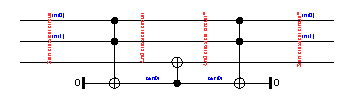
\includegraphics[width=.85\textwidth]{img/circuito}
\end{columns}


\end{frame}

\subsection{Algoritmo de Deutsch-Jozsa}

\begin{frame}[fragile]{Algoritmo de Deutsch-Jozsa}

  Determina en una consulta si un predicado es constante o balanceado.

\begin{lstlisting}
deutschJozsa :: (QShape ba qa ca) => Oracle qa -> Circ ca
\end{lstlisting}

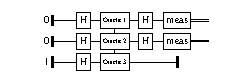
\includegraphics[width=\textwidth]{img/deutsch}

Si el predicado es balanceado la amplitud del estado $\ket{0\dots 0}$ se anula,
y si es constante se hace $\pm1$.

\note{El caso clásico se hace en $O(N)$}

\end{frame}

\subsection{Algoritmo de Shor}

\begin{frame}[fragile]{Transformada cuántica de Fourier}

  Hace la DFT normalizada sobre las amplitudes en $O((\log N)^2)$ pasos.

\begin{lstlisting}
qft :: [Qubit] -> Circ [Qubit]
qft []     = pure []
qft (x:xs) = do
  xs'  <- qft xs
  xs'' <- rotations x xs' (length xs')
  x'   <- hadamard x
  pure (x' : xs'')
\end{lstlisting}
  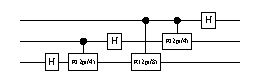
\includegraphics[width=\textwidth]{img/qft}
\end{frame}

\begin{frame}{Algoritmo de estimación de fase}
  Estima el autovalor asociado a un autovector de un operador unitario en $O((\log N)^2)$ pasos.

  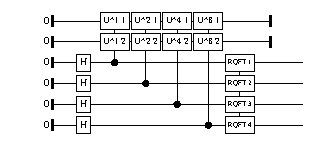
\includegraphics[width=\textwidth]{img/qpe}

  Utiliza la transformada de Fourier cuántica inversa.
\end{frame}

\begin{frame}[fragile]{Algoritmo de Shor}

  El algoritmo de Shor transforma la factorización de $N$ en el problema de
  hallar el orden de una unidad $x \in U(\ZZ_N)$ en tiempo $O((\log N)^3)$.

  La simulación no es factible en la práctica; implemento la parte clásica y estimo los recursos para la parte
  cuántica si hiciera falta.

  \begin{lstlisting}
operador :: Integer -> Integer -> Int -> QDInt -> Circ QDInt
operador x n j y = do
  q_n           <- qinit (toIntM n)
  (y, z)        <- q_mult_param a y -- x^j mod n * y
  (z, q_n, res) <- q_mod_unsigned z q_n
  pure res -- x^j*y mod n
where a = toIntM (binaryExp x (fromIntegral j) n)
  \end{lstlisting}
  
\includegraphics[width=\textwidth]{img/shor}
\end{frame}

\subsection{Algoritmo de Grover}

\begin{frame}[fragile]{Algoritmo de Grover}
  Encuentra una solución a $f(x) = 1$ en $O\left(\sqrt{N}\right)$ consultas a $f$.

  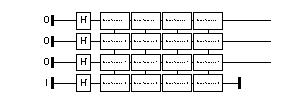
\includegraphics[width=\textwidth]{img/grover}

  Se basa en la rotación adecuada de un vector en un plano del espacio de estados.
  Es factible simularlo en casos pequeños.

  Puede apoyarse en el \emph{algoritmo de conteo cuántico}.

\end{frame}

\begin{frame}[fragile]{Operador de Grover}

  El oráculo refleja $$\ket{x} \mapsto (-1)^{f(x)}\ket{x}$$
  mientras que el operador \texttt{phaseShift} refleja $$\ket{x} \mapsto (-1)^{\delta_{x0}}\ket{x}.$$
  Esto nos da una rotación.

  \begin{lstlisting}
diffusion :: [Qubit] -> Circ [Qubit]
diffusion = map_hadamard >=> phaseShift >=> map_hadamard

groverOperator ::
   Oracle [Qubit] -> ([Qubit], Qubit) -> Circ ([Qubit], Qubit)
groverOperator oracle (xs, y) = do
  (xs, y) <- circuit oracle (xs, y)
  xs      <- diffusion xs
  pure (xs, y)
\end{lstlisting}
\end{frame}


\begin{frame}{Conclusiones}
  \begin{itemize}[<+->]
  \item Los últimos 25 años han supuesto grandes avances en la teoría de la complejidad cuántica, que tiene profundas relaciones con el ámbito clásico; la demostración de la supremacía cuántica resolvería el problema $\mathsf{P} \qeq \mathsf{PSPACE}.$
  \item Los lenguajes de programación cuánticos permiten expresar los algoritmos presentes en la literatura de forma concisa, pero trabajan aún a muy bajo nivel y no hay consenso respecto de las estructuras de control básicas.
  \end{itemize}
\end{frame}

\begin{frame}[standout]

Gracias por su atención
\end{frame}

\end{document}
